\documentclass[]{article}

% Imported Packages
%------------------------------------------------------------------------------
\usepackage{amssymb}
\usepackage{amstext}
\usepackage{amsthm}
\usepackage{amsmath}
\usepackage{enumerate}
\usepackage{fancyhdr}
\usepackage[margin=1in]{geometry}
\usepackage{graphicx}
\usepackage{extarrows}
\usepackage{setspace}
\numberwithin{figure}{section}
%------------------------------------------------------------------------------

% Header and Footer
%------------------------------------------------------------------------------
\pagestyle{plain}  
\renewcommand\headrulewidth{0.4pt}                                      
\renewcommand\footrulewidth{0.4pt}                                    
%------------------------------------------------------------------------------

% Title Details
%------------------------------------------------------------------------------
\title{Deliverable \#3 Template}
\author{SE 3A04: Software Design II -- Large System Design}
\date{}                               
%------------------------------------------------------------------------------

% Document
%------------------------------------------------------------------------------
\begin{document}

\maketitle	
\noindent{\bf Tutorial Number:} T01\\
{\bf Group Number:} G08 \\
{\bf Group Members:} 
\begin{itemize}
	\item Patolia, Yash
	\item Wang, Jasmine
	\item Kwinecki, Justin Joseph
	\item Zhang, Christina
	\item Huzaifah, Muhammad
	\item Hum, Nathan Joshua
\end{itemize}

\clearpage
\section{Introduction}
\label{sec:introduction}
% Begin Section

This section should provide an brief overview of the entire document.

\subsection{Purpose}
\label{sub:purpose}
% Begin SubSection
This document provides more details on the Nutrify system architecture, including state chart diagrams, sequence diagrams, and a detailed class diagram. It's meant for internal Nutrify stakeholders, such as project managers, developers, domain experts, and team members/investors.  Deliverables 1 and 2 provide an in-depth background and provide more insight in the decisions leading up to this document and should be reviewed prior.
% End SubSection

\subsection{System Description}
\label{sub:system_description}
% Begin SubSection
A brief overview of the system description can be found in deliverable 2. This document acts as an extension of deliverable 2 and provides more context in forms of state charts, sequence diagrams and a detailed class diagram.
% End SubSection

\subsection{Overview}
\label{sub:overview}
% Begin SubSection
This document is organized by chart / diagram type. Section 2 contains relevant state charts for controller classes, section 3 contains relevant sequence diagrams and section 4 contains a detailed UML diagram of the system.

% End SubSection

% End Section

\clearpage
\section{State Charts for Controller Classes}
\label{sec:state_charts_for_controller_classes}
% Begin Section
\begin{figure}[h]
    \centering
    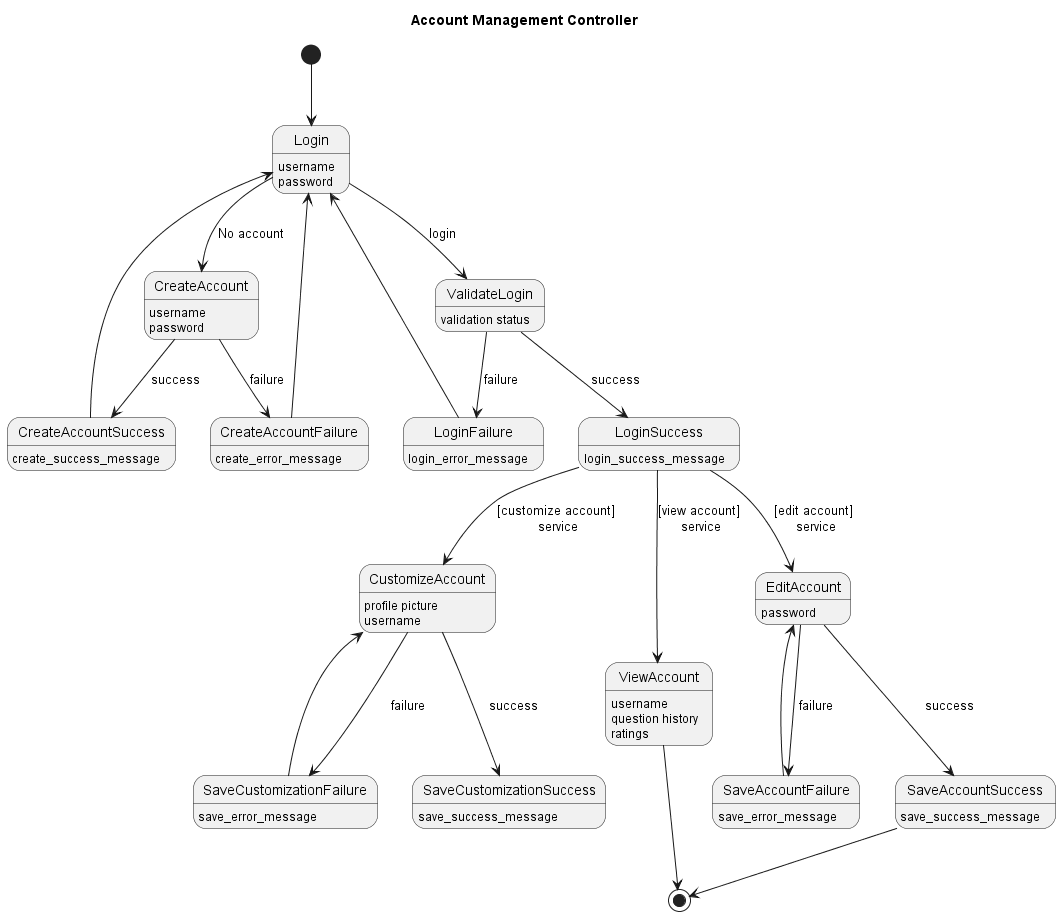
\includegraphics[width=1\textwidth]{diagrams/state/accountstate.png} % Adjust width as needed
    \caption{Account Management Controller State Diagram}
\end{figure}

\begin{figure}[h]
    \centering
    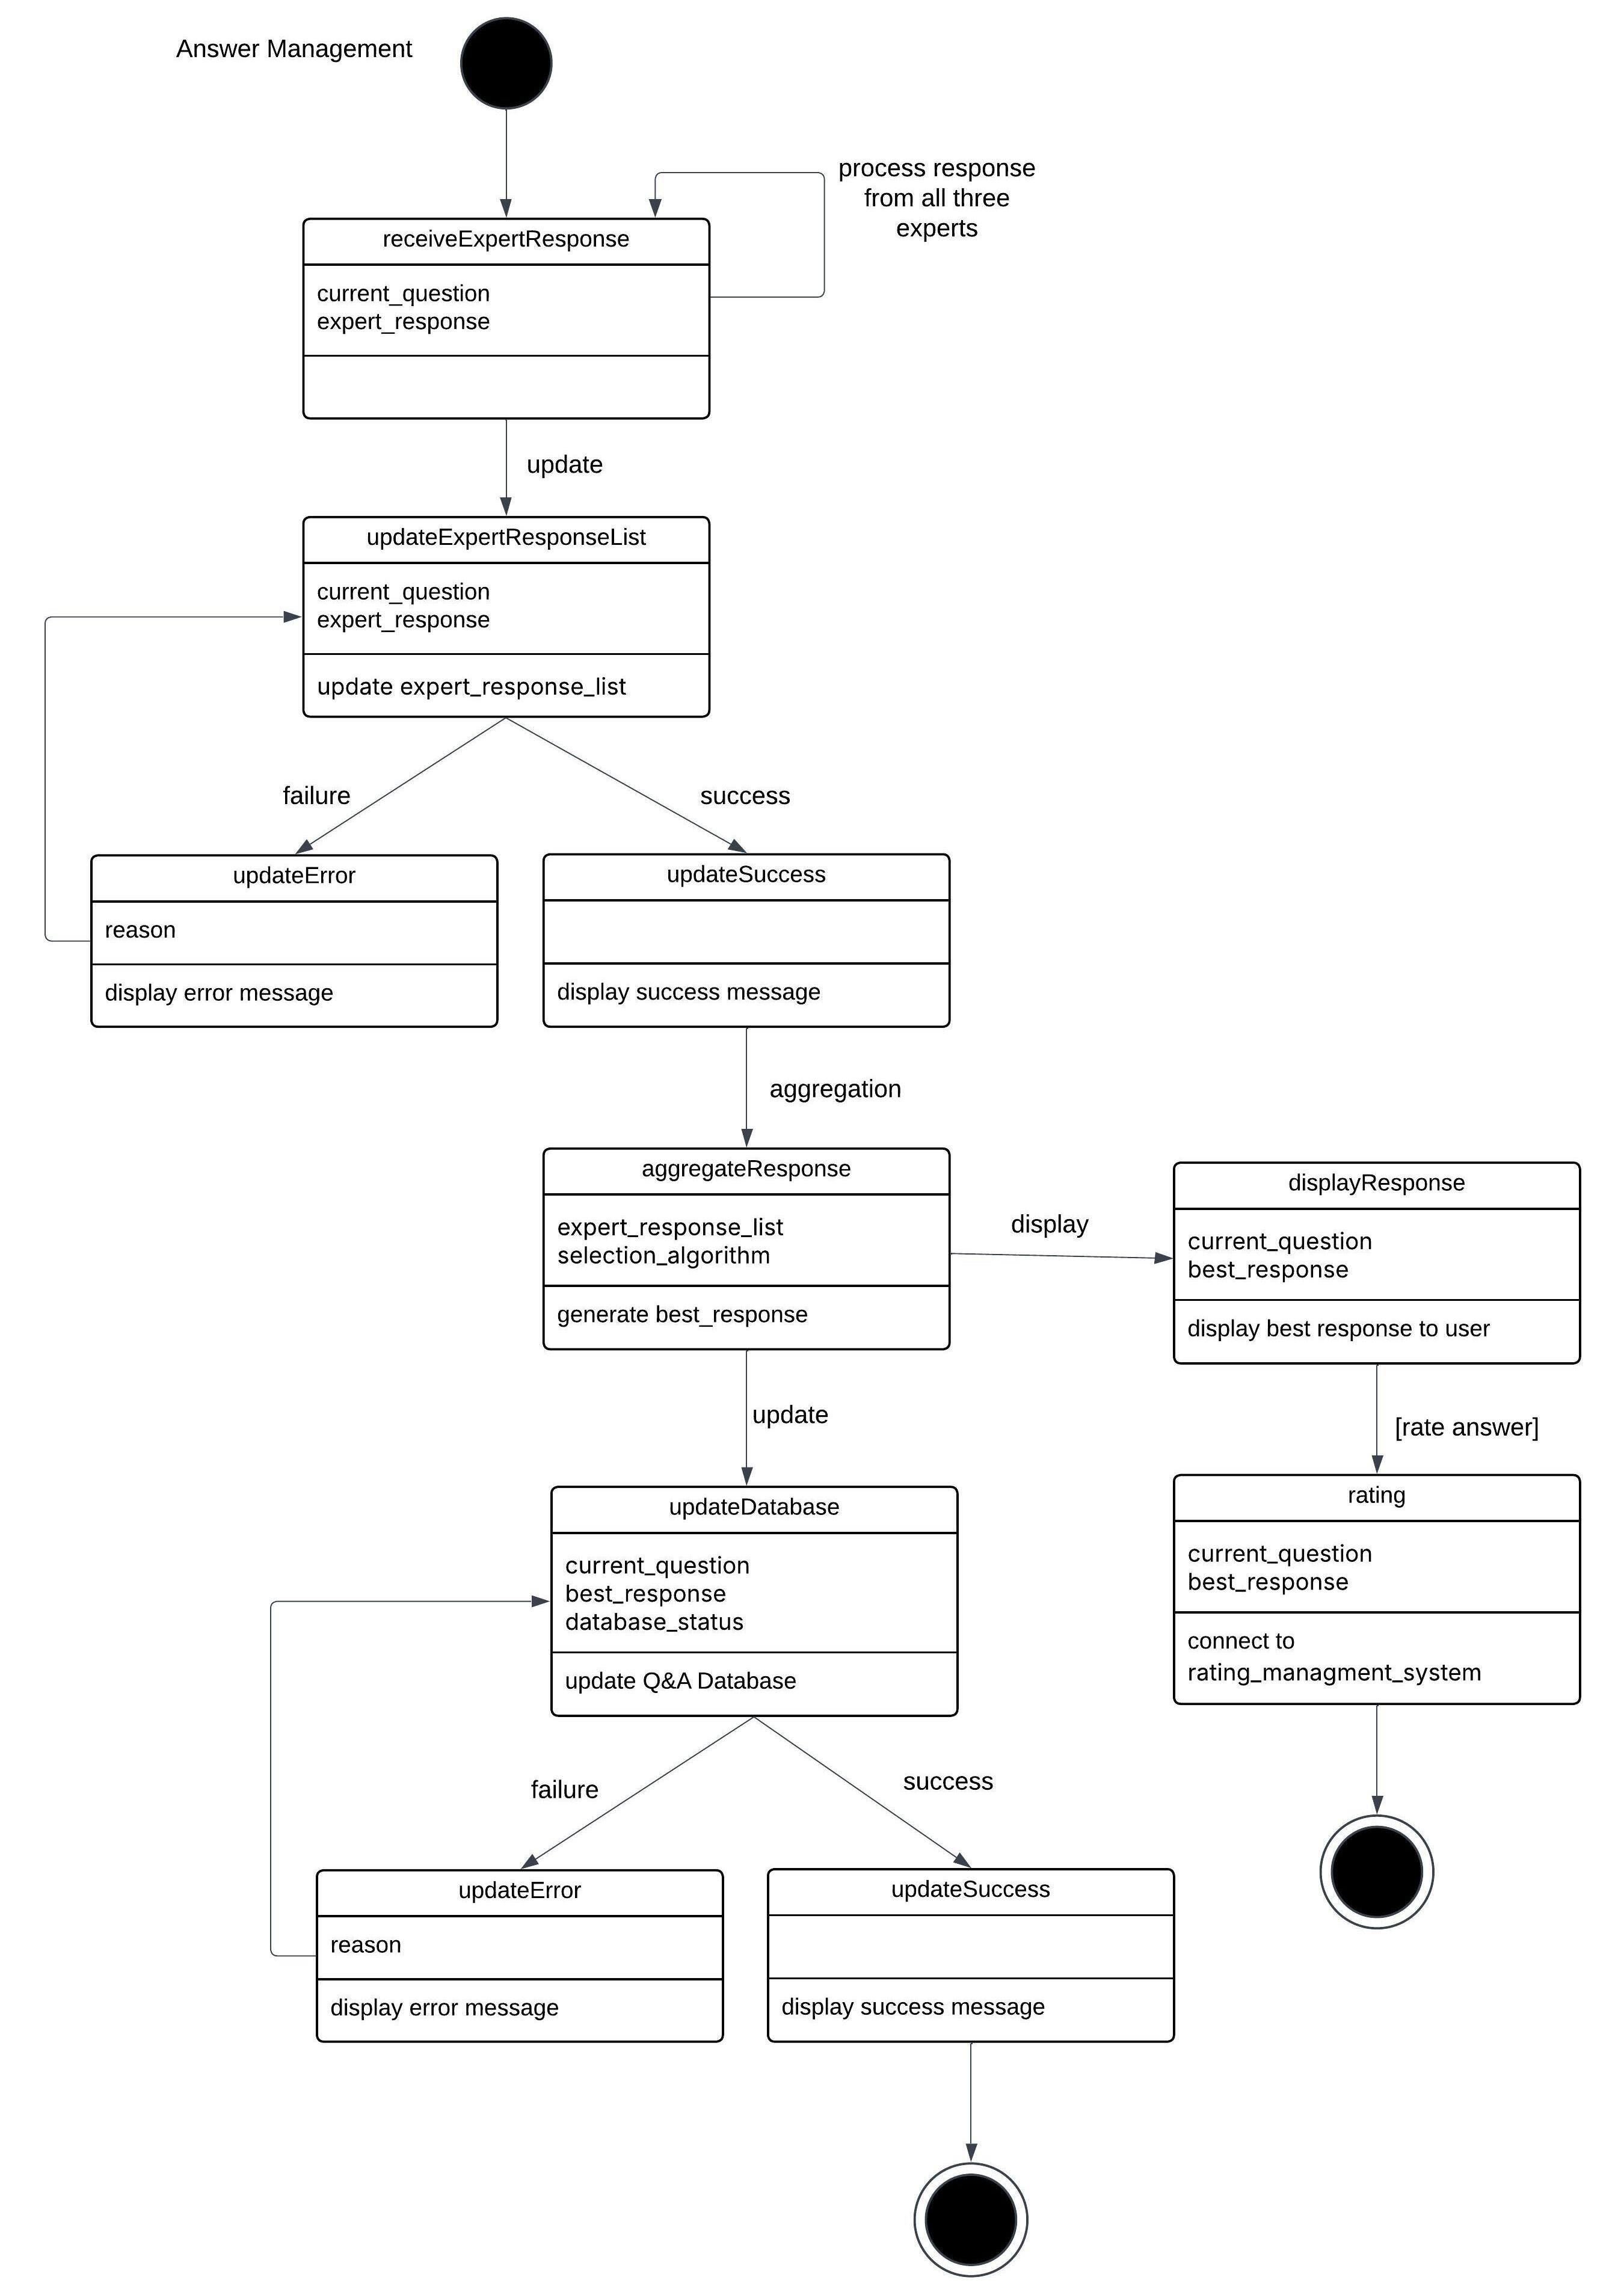
\includegraphics[width=0.8\textwidth]{diagrams/state/AnswerStateDiagram.jpeg} % Adjust width as needed
    \caption{Answer Management Controller State Diagram}
\end{figure}

\begin{figure}[h]
    \centering
    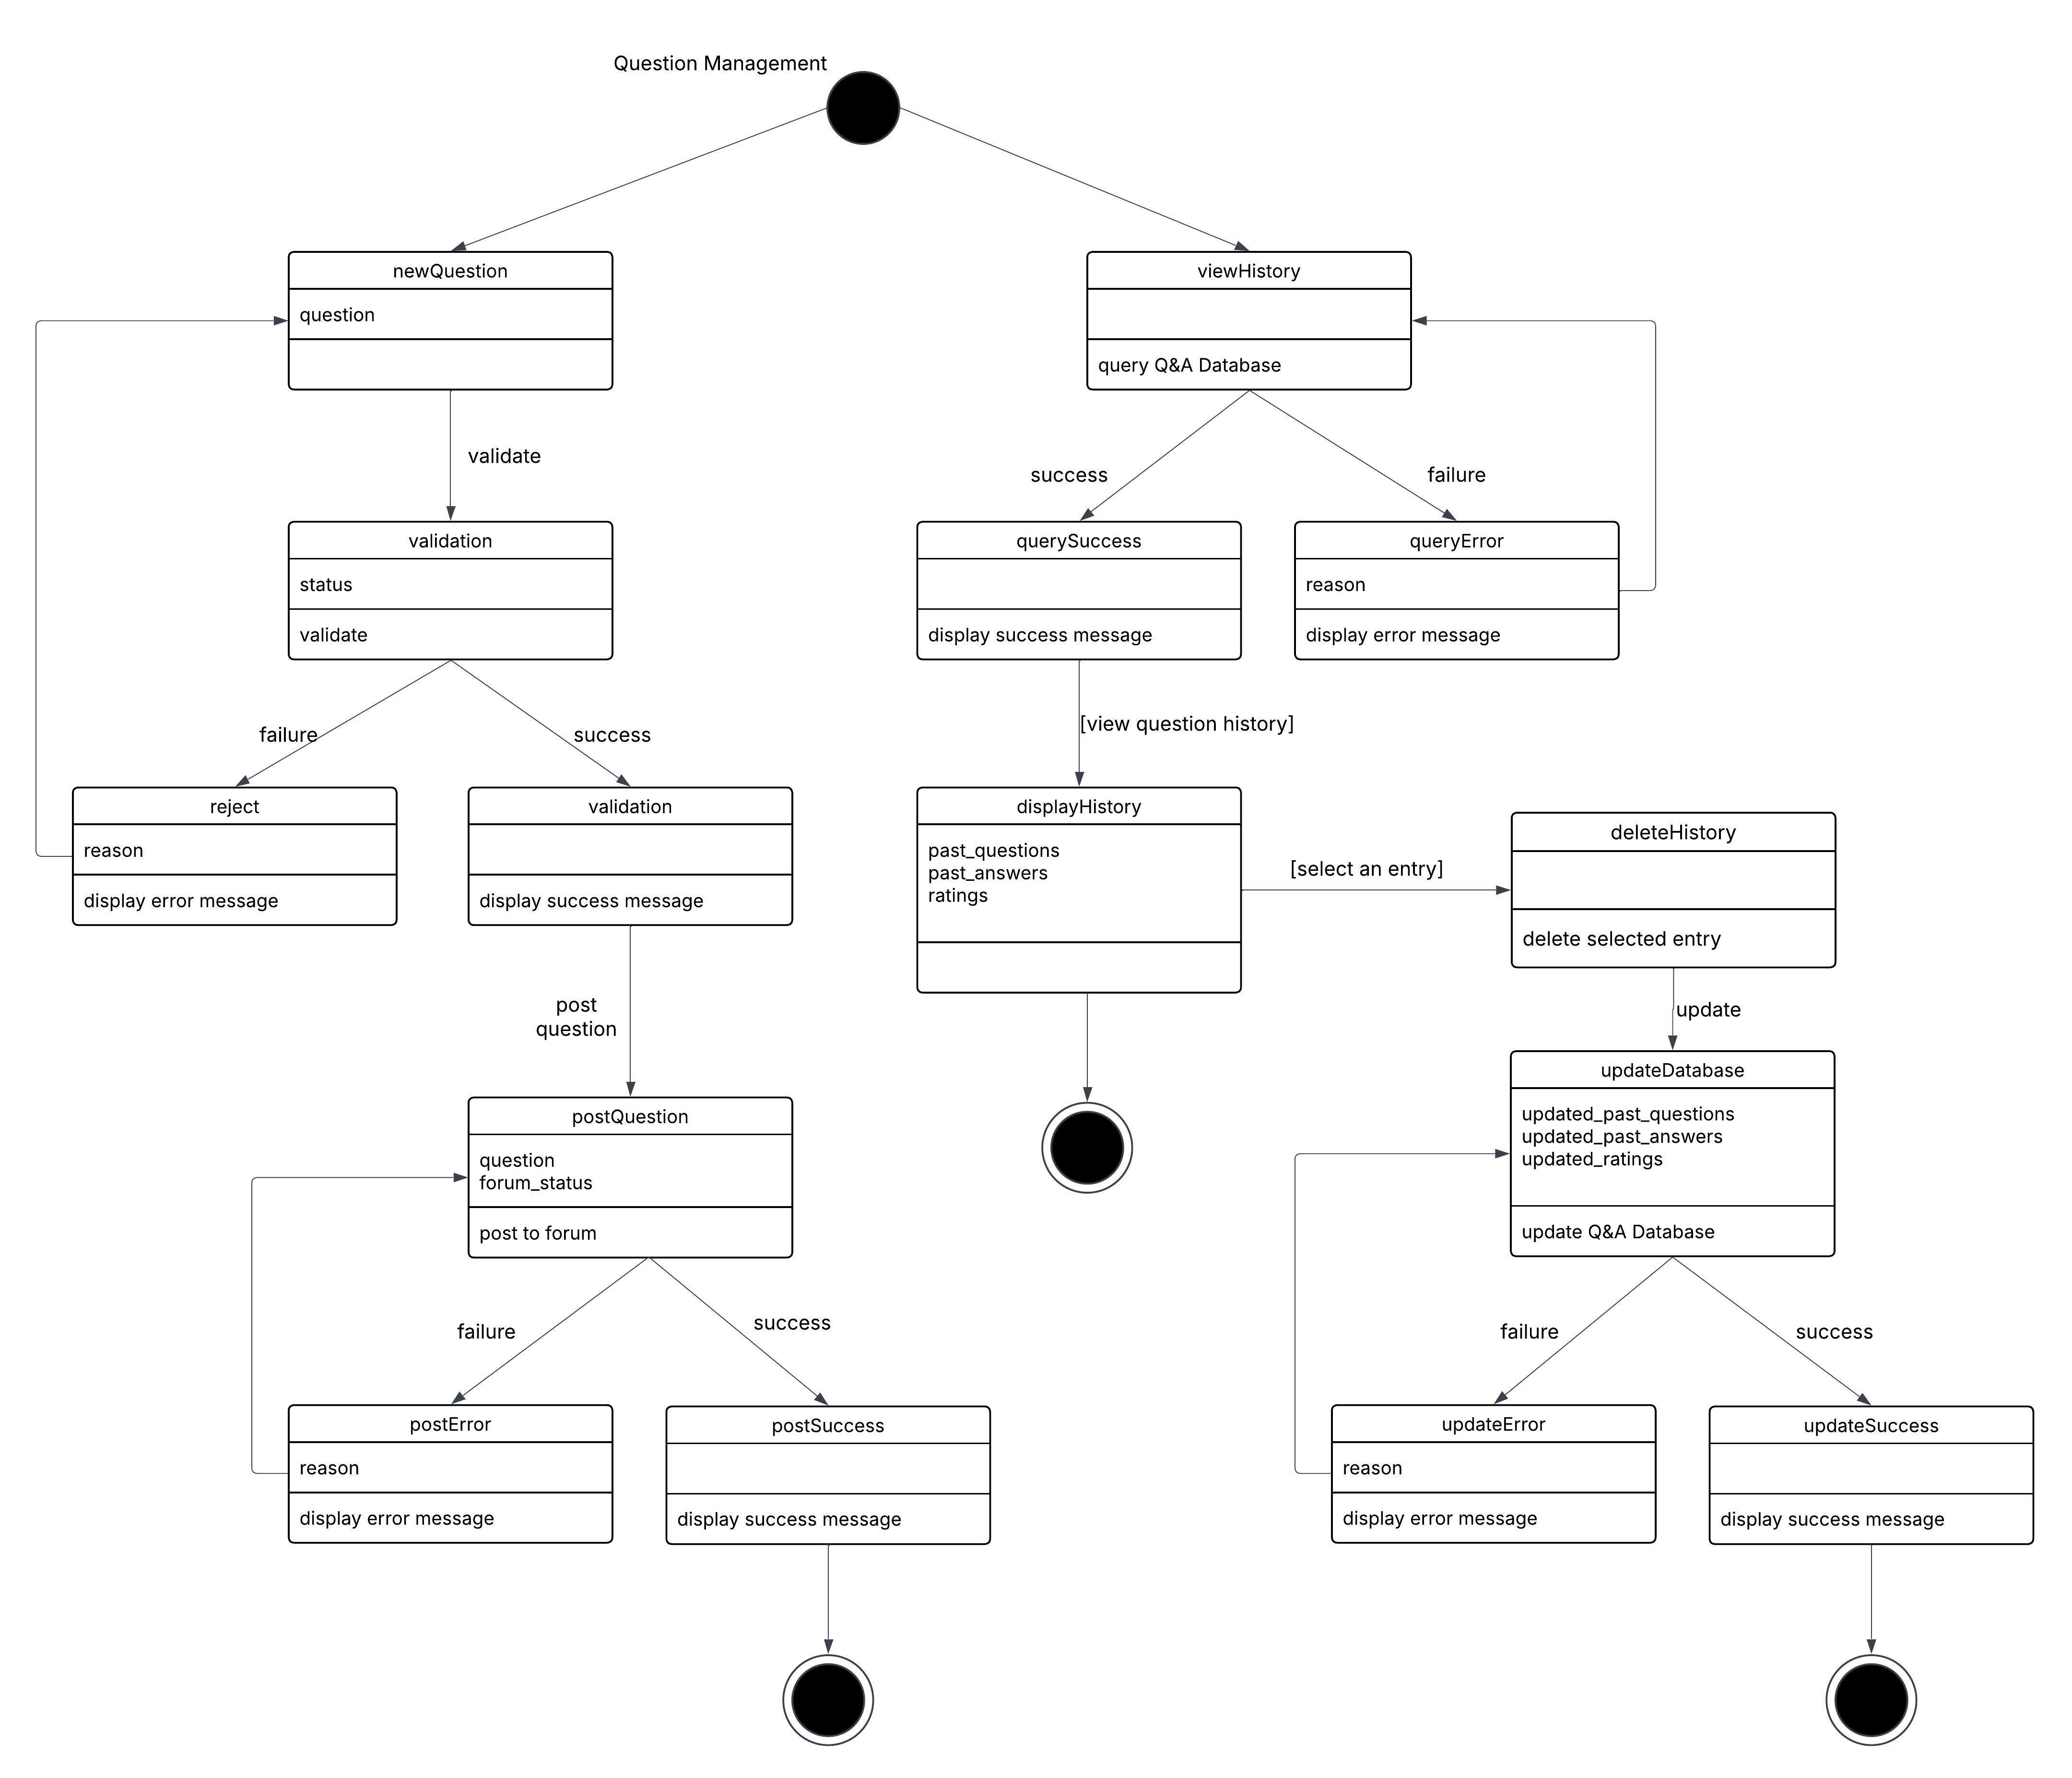
\includegraphics[width=1\textwidth]{diagrams/state/QuestionStateDiagram.jpeg} % Adjust width as needed
    \caption{Question Management Controller State Diagram}
\end{figure}

\begin{figure}[h]
    \centering
    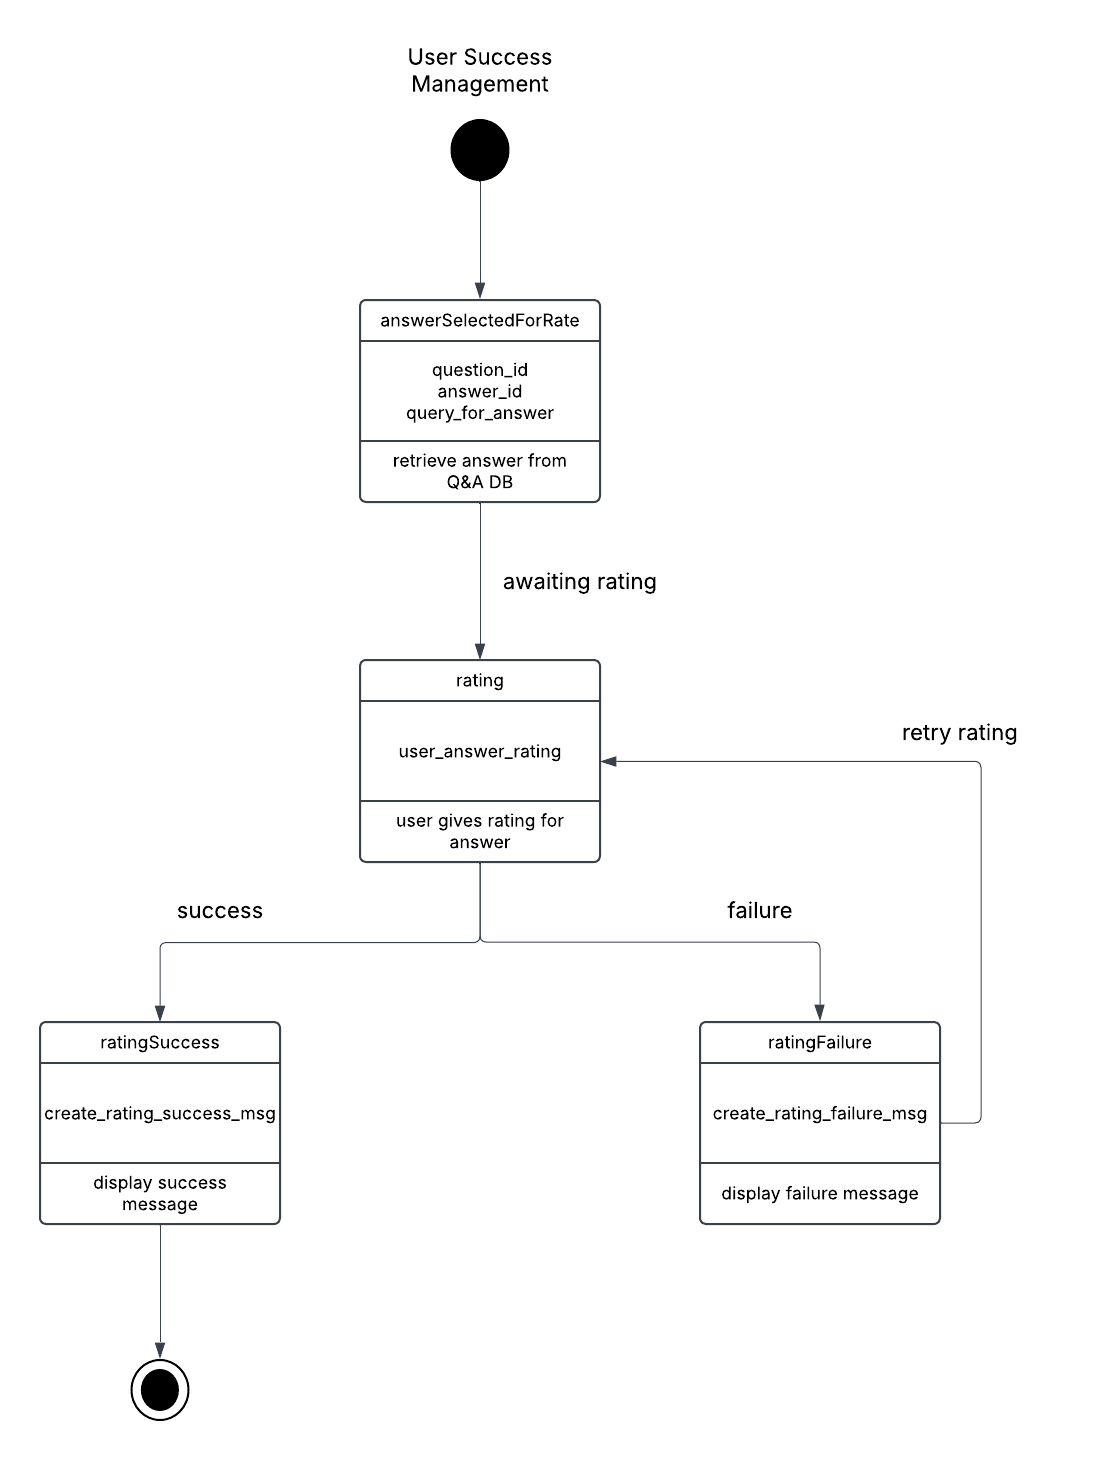
\includegraphics[width=0.8\textwidth]{diagrams/state/UserSuccessState.png} % Adjust width as needed
    \caption{User Success Management Controller State Diagram}
\end{figure}
% End Section

\clearpage
\section{Sequence Diagrams}
\label{sec:sequence_diagrams}
% Begin Section
\begin{figure}[ht]
    \centering
    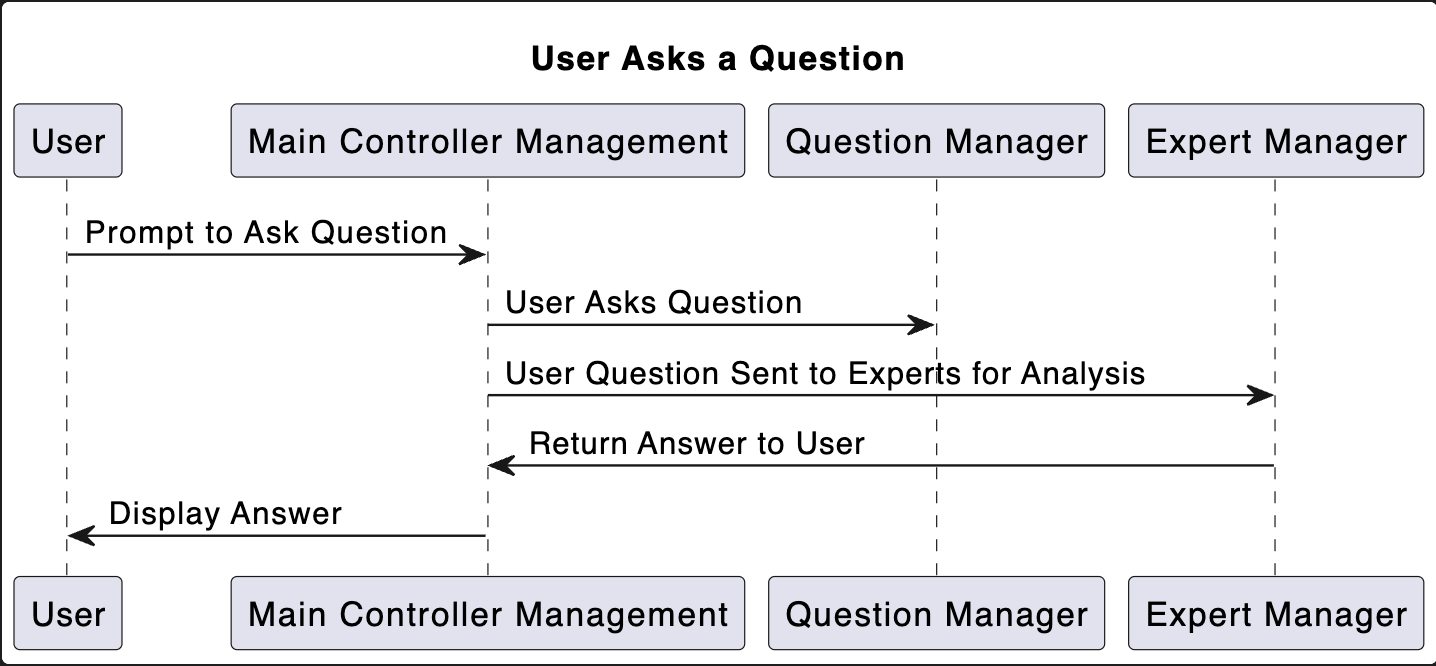
\includegraphics[width=0.7\textwidth]{diagrams/sequence/AskQuestionSequence.png} % Adjust width as needed
    \caption{Ask Question Sequence Diagram}
\end{figure}

\begin{figure}[ht]
    \centering
    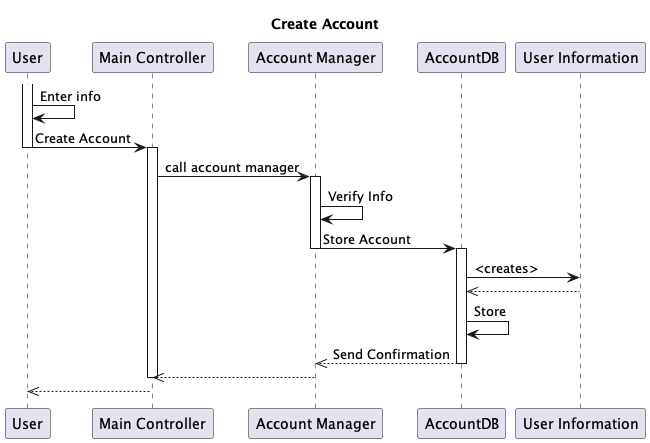
\includegraphics[width=0.7\textwidth]{diagrams/sequence/create_account.png} % Adjust width as needed
    \caption{Create Account Sequence Diagram}
\end{figure}

\begin{figure}[ht]
    \centering
    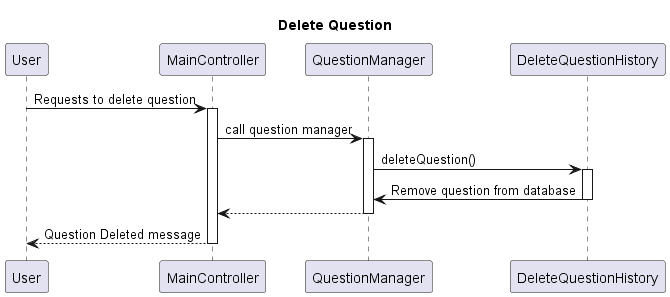
\includegraphics[width=0.7\textwidth]{diagrams/sequence/deleteqsequence.png} % Adjust width as needed
    \caption{Delete Question Sequence Diagram}
\end{figure}

\begin{figure}[ht]
    \centering
    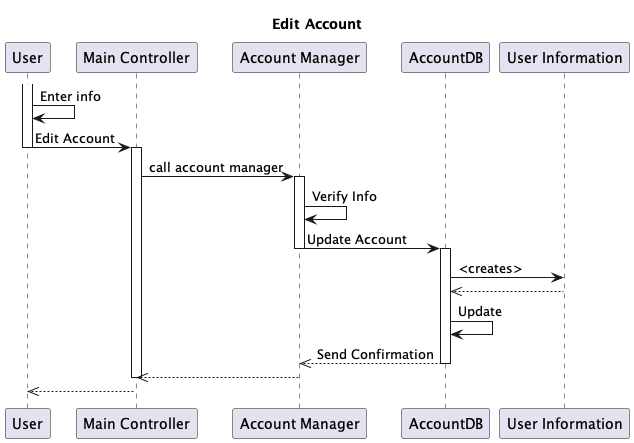
\includegraphics[width=0.7\textwidth]{diagrams/sequence/edit_account.png} % Adjust width as needed
    \caption{Edit Account Sequence Diagram}
\end{figure}
% End Section

\clearpage
\section{Detailed Class Diagram}
\label{sec:detailed_class_diagram}
% Begin Section
\begin{figure}[h]
    \centering
    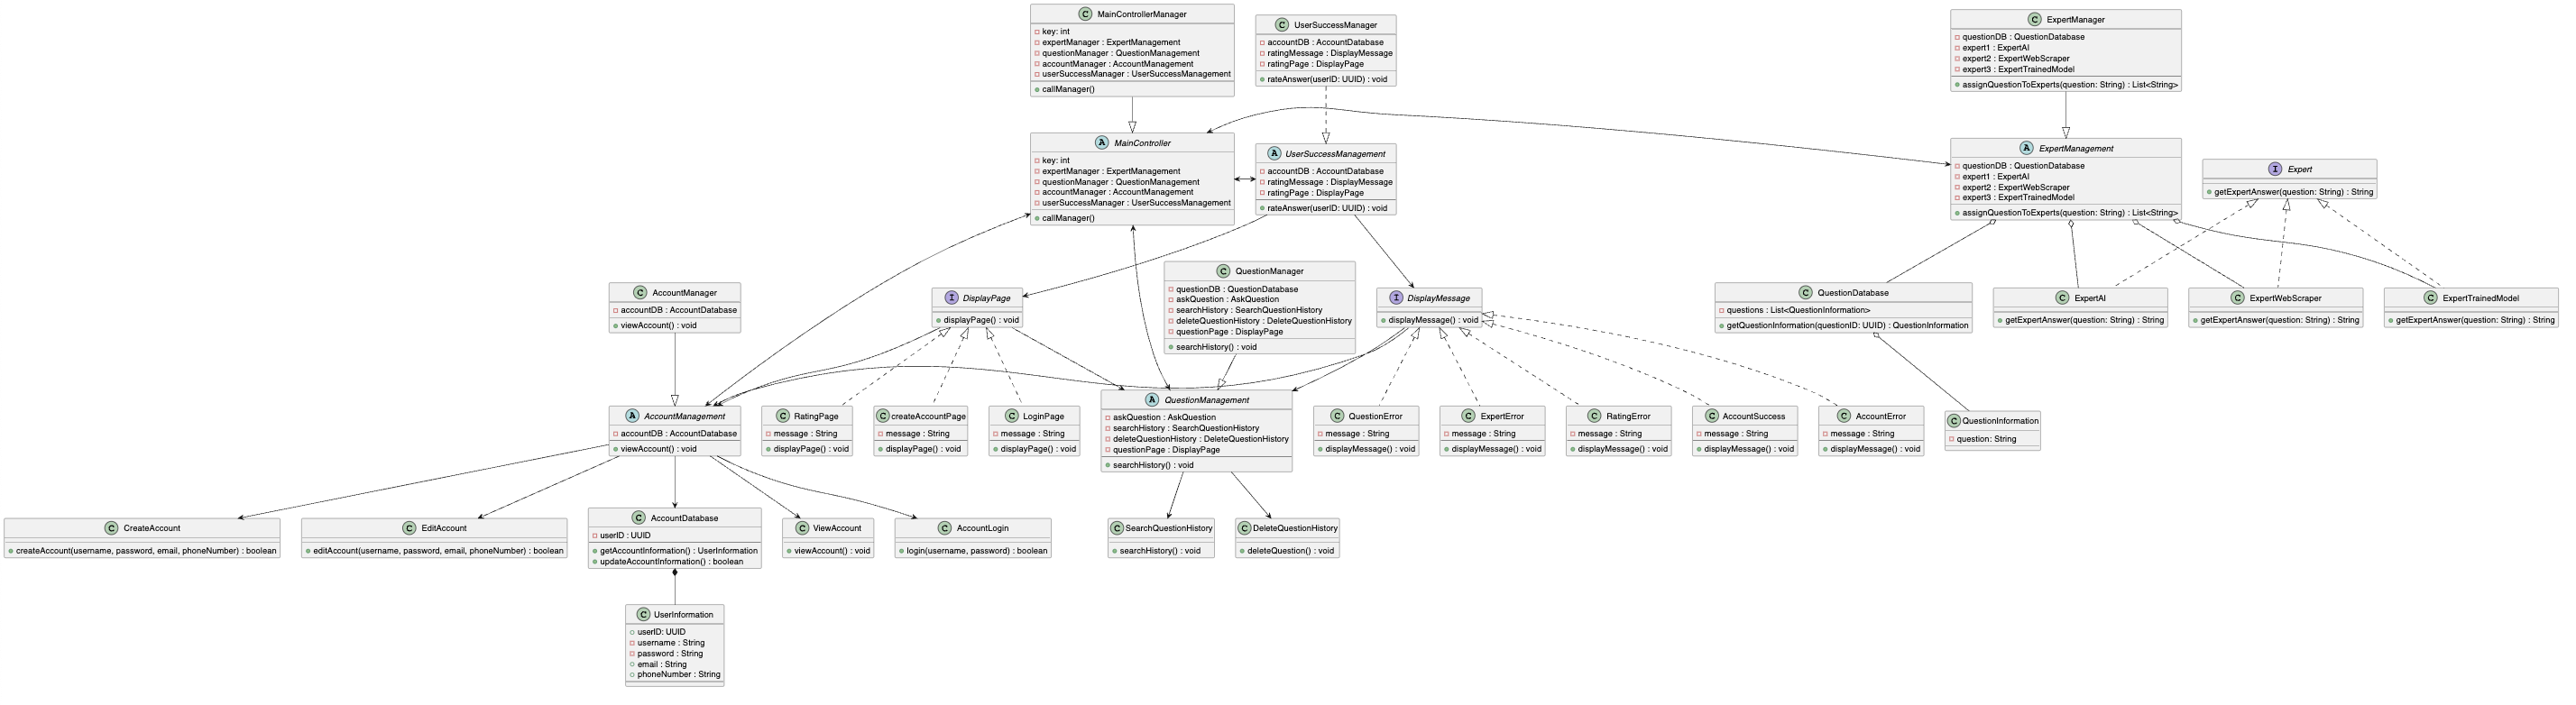
\includegraphics[width=1\textwidth]{diagrams/classdiagram.png} % Adjust width as needed
    \caption{Overall Detailed Class Diagram}
\end{figure}

\begin{figure}[h]
    \centering
    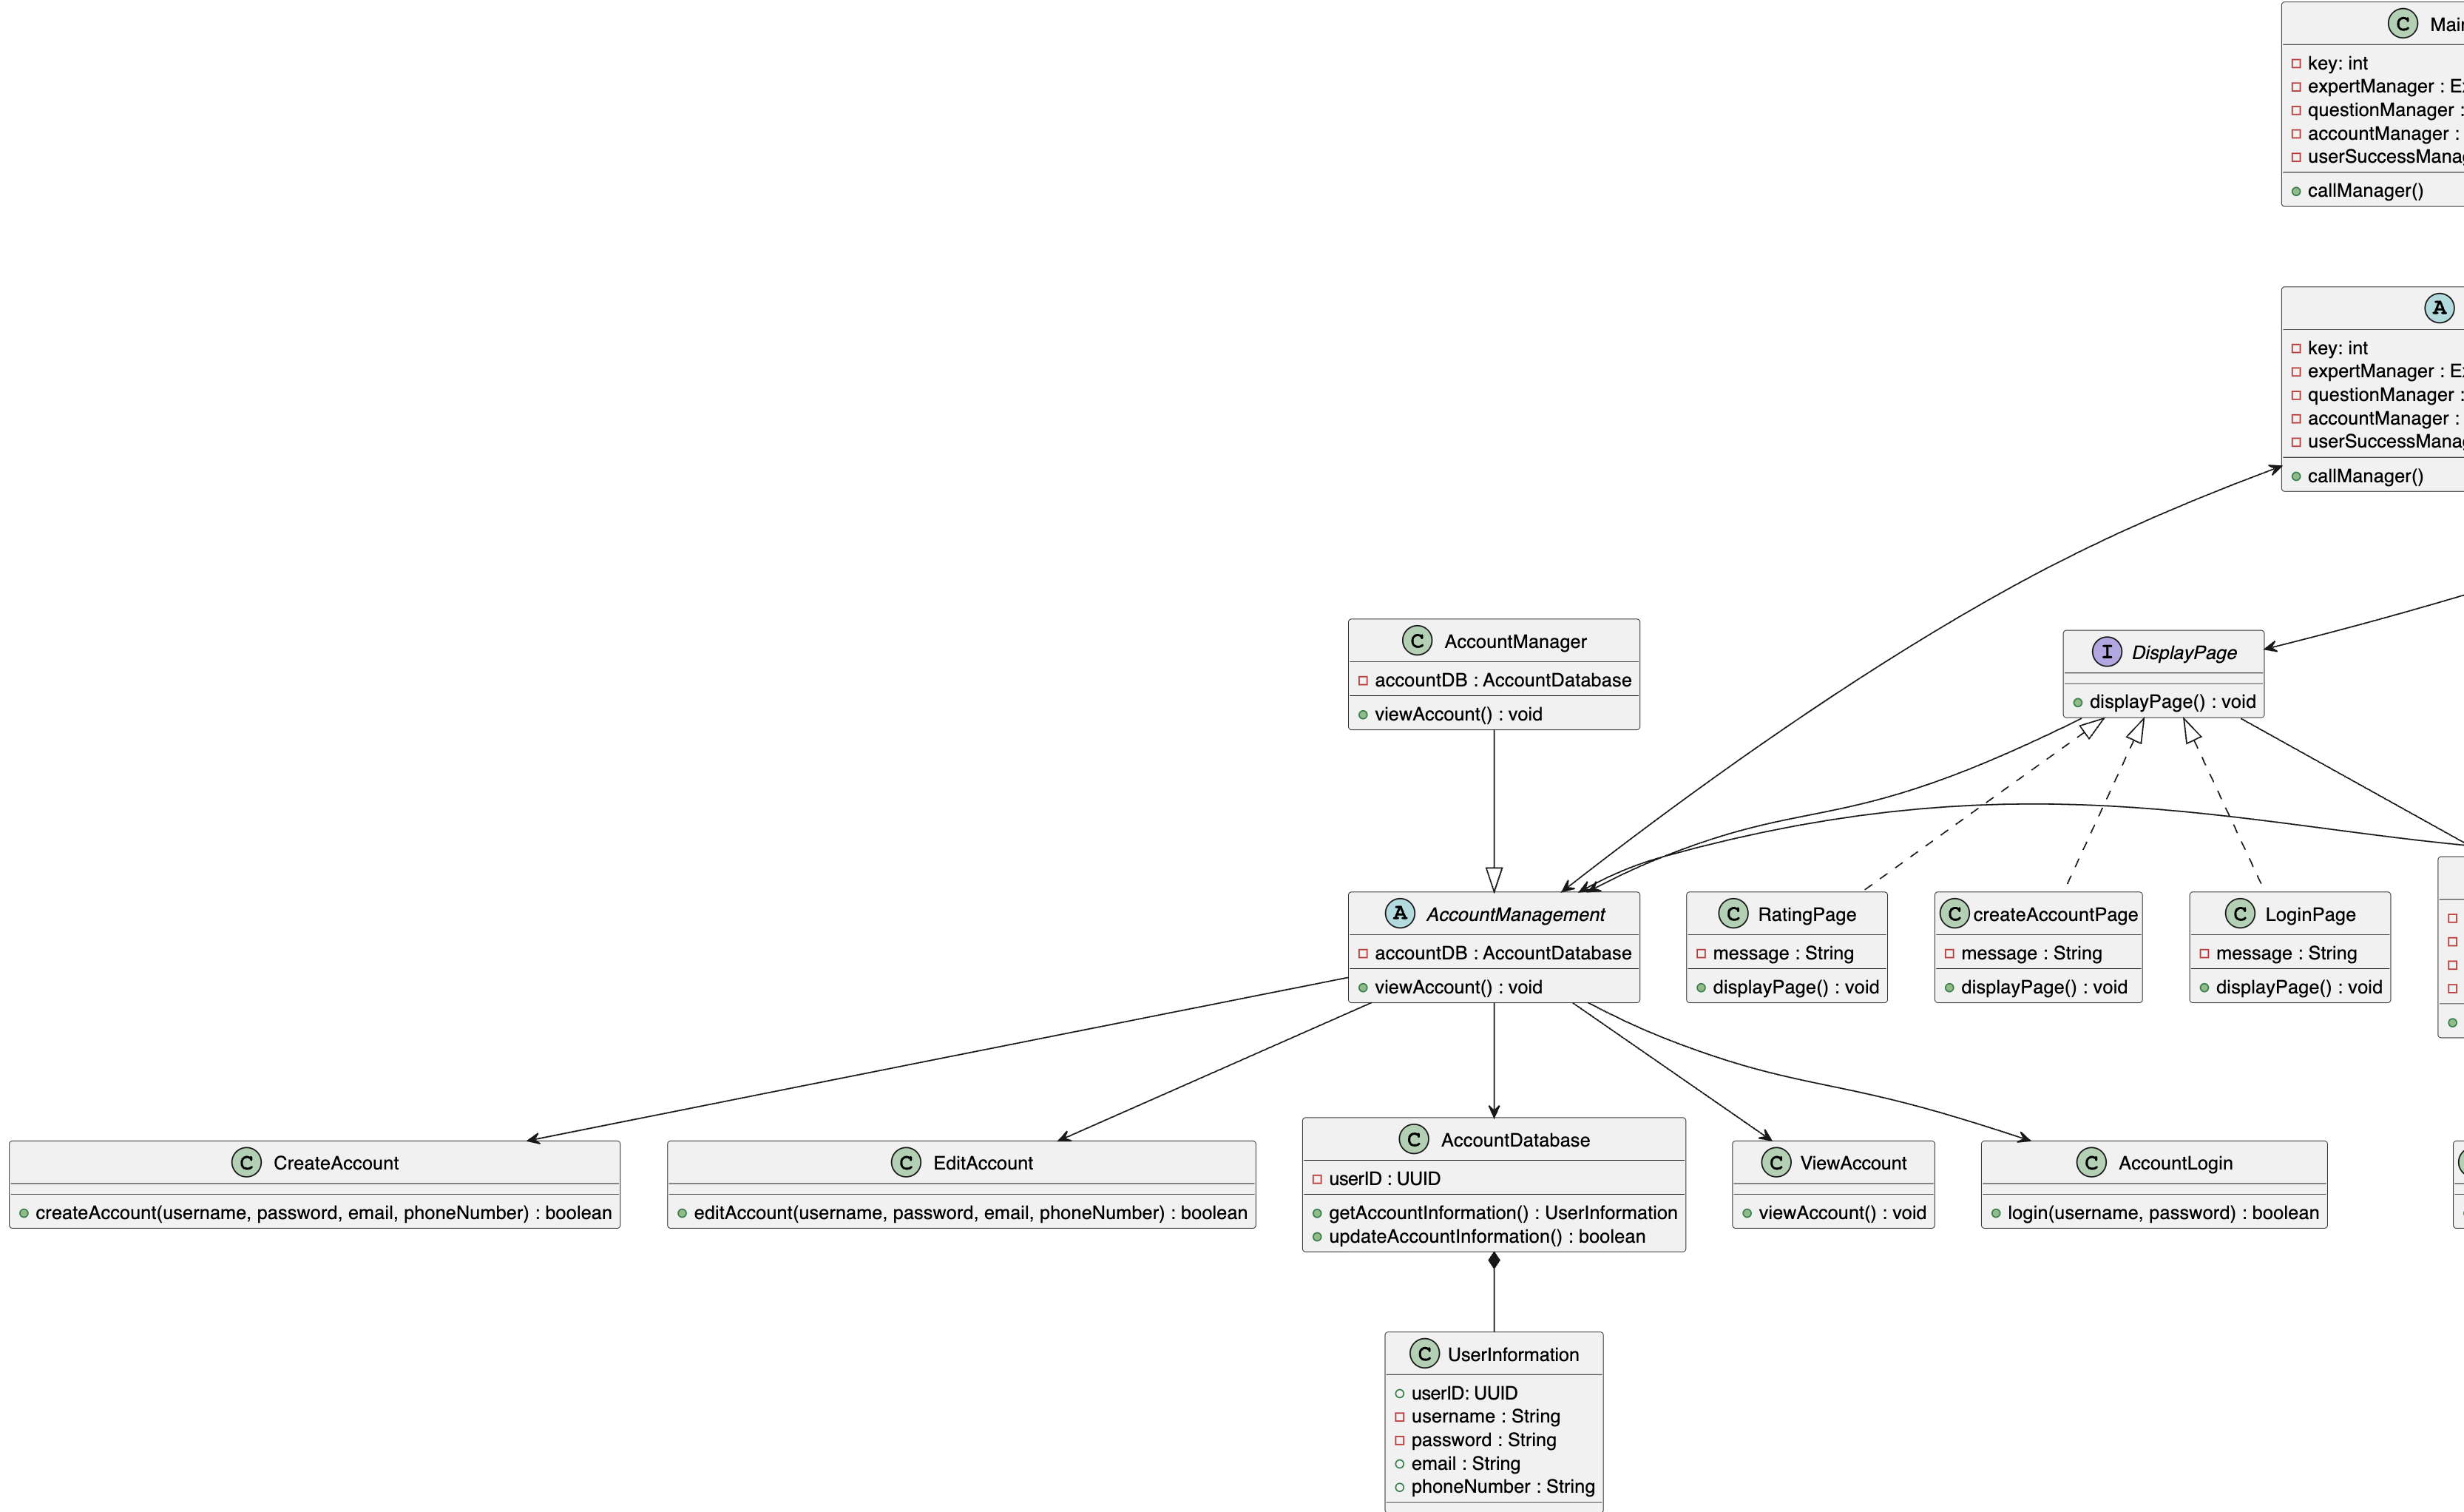
\includegraphics[width=1\textwidth]{diagrams/left.png} % Adjust width as needed
    \caption{Detailed Class Diagram 1 (Left)\\}
\end{figure}

\begin{figure}[h]
    \centering
    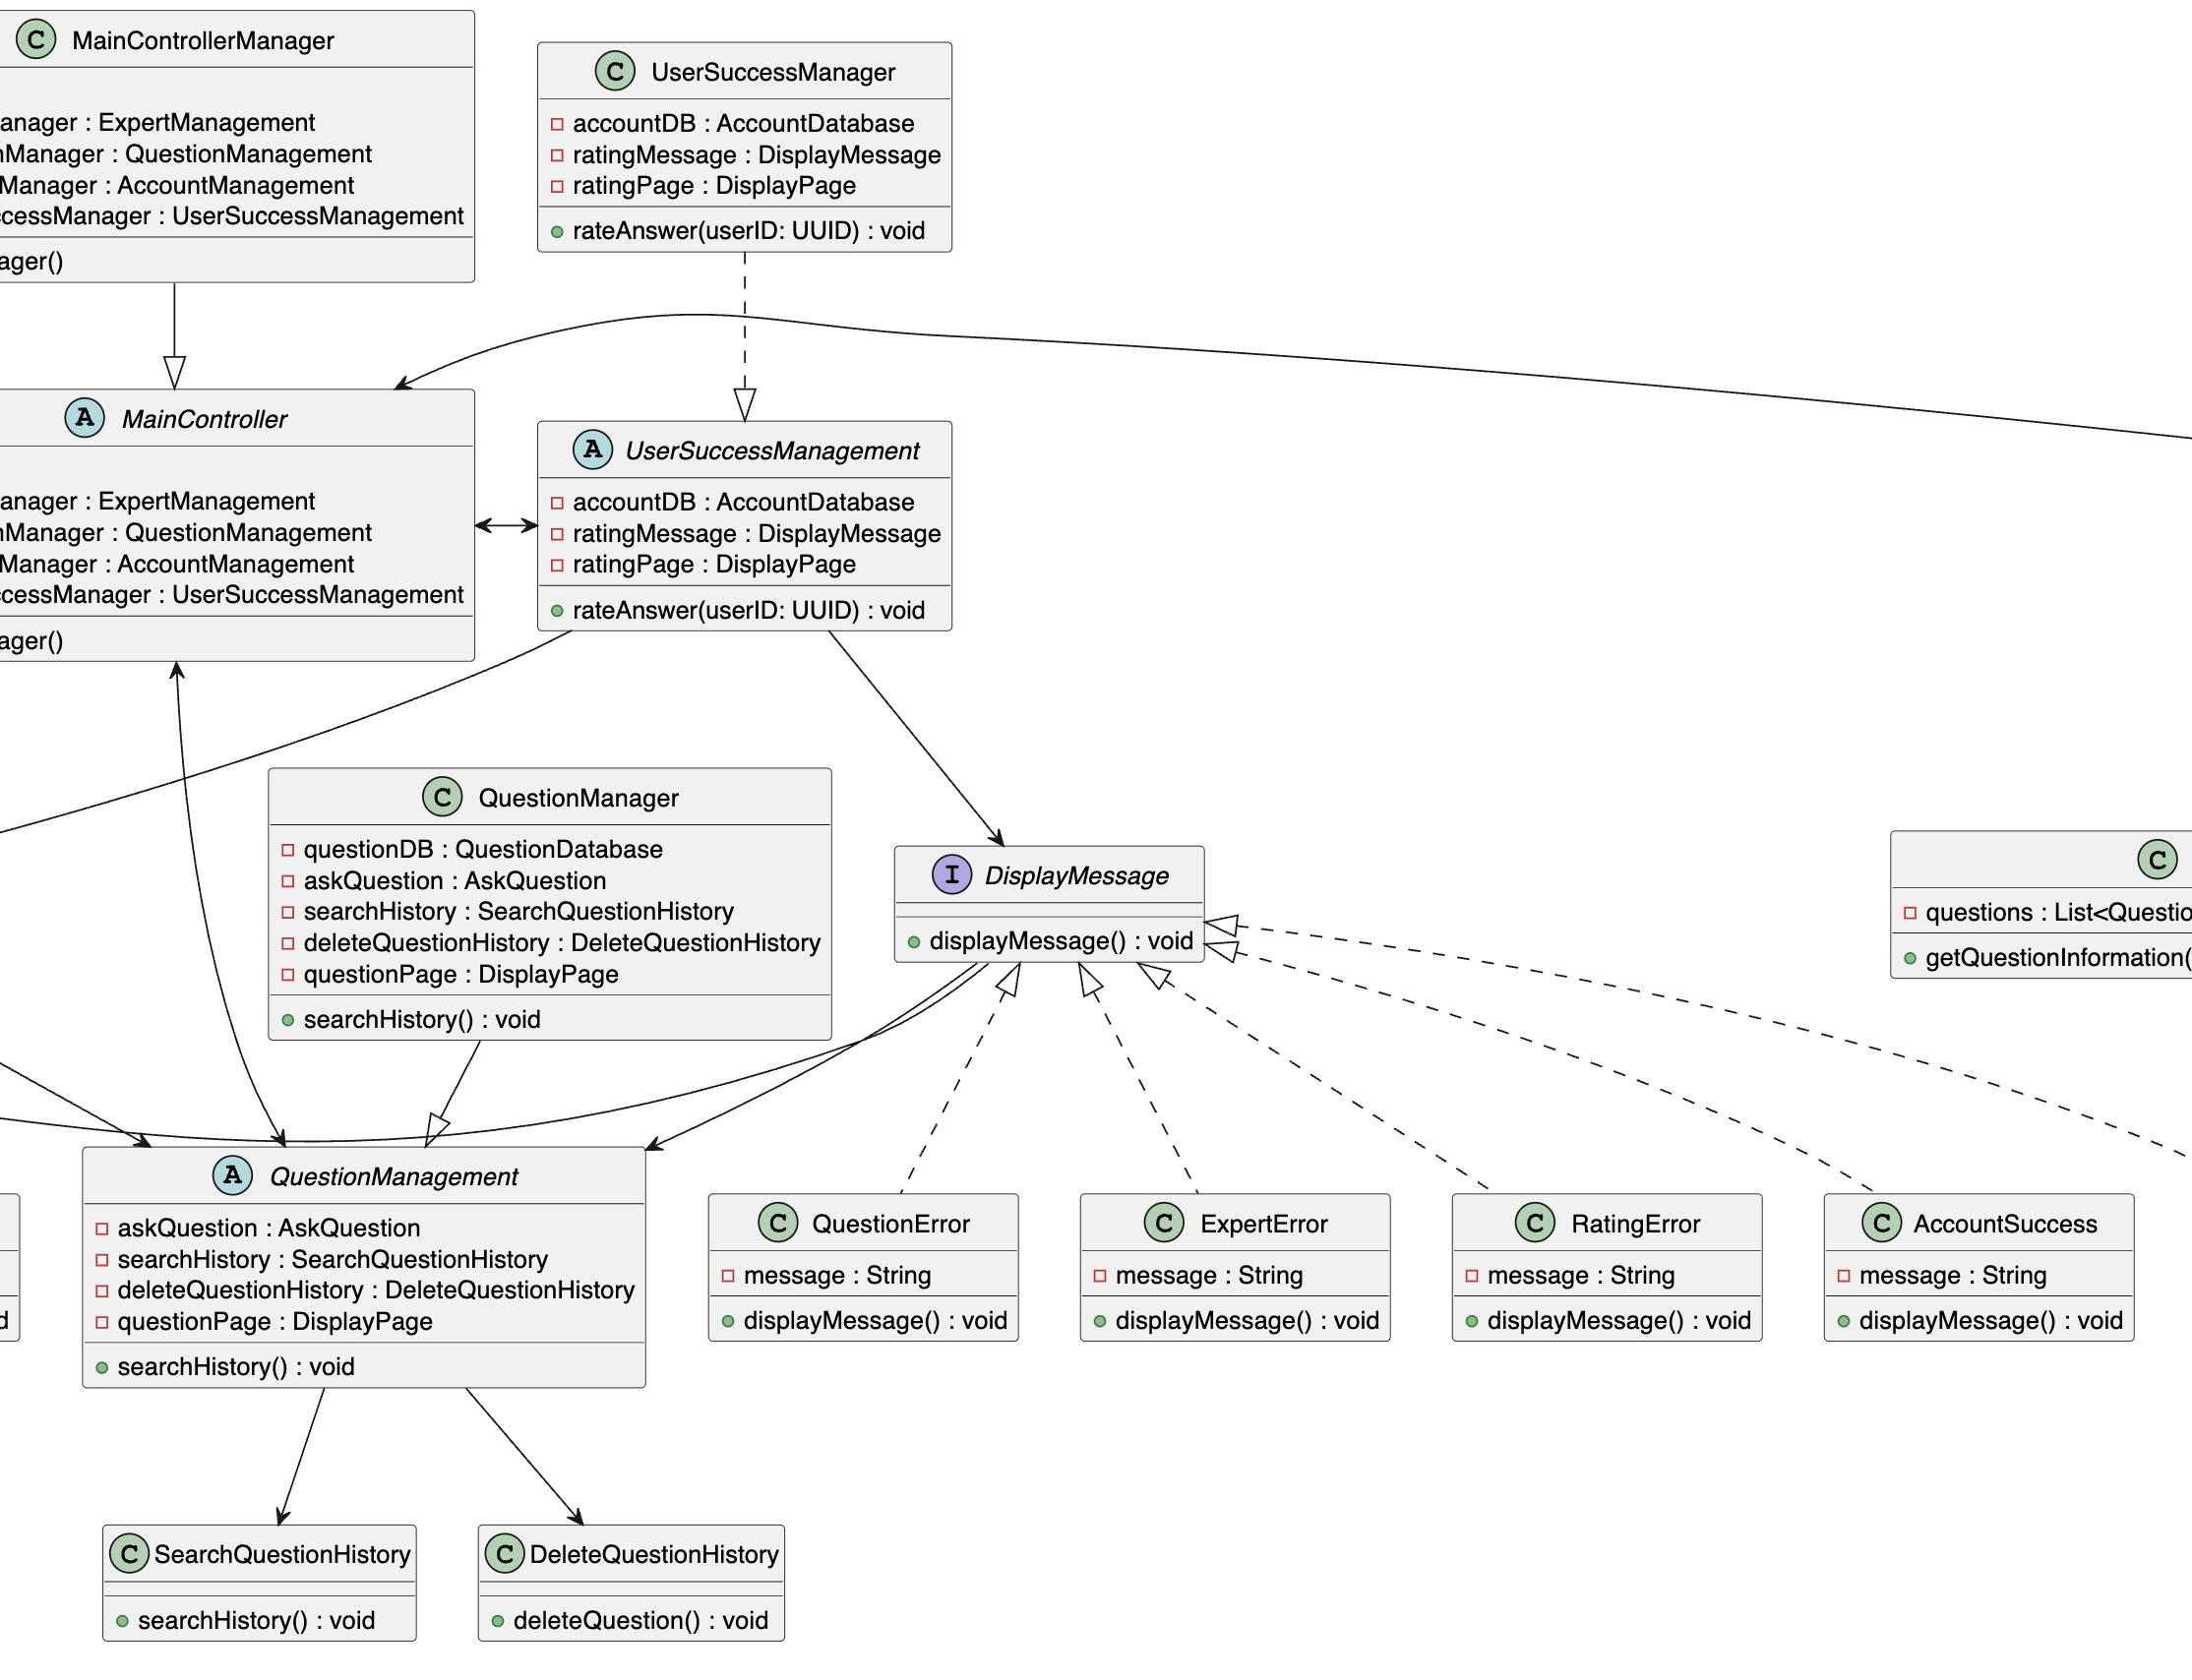
\includegraphics[width=1\textwidth]{diagrams/middle.png} % Adjust width as needed
    \caption{Detailed Class Diagram 2 (Middle)\\}
\end{figure}

\begin{figure}[h]
    \centering
    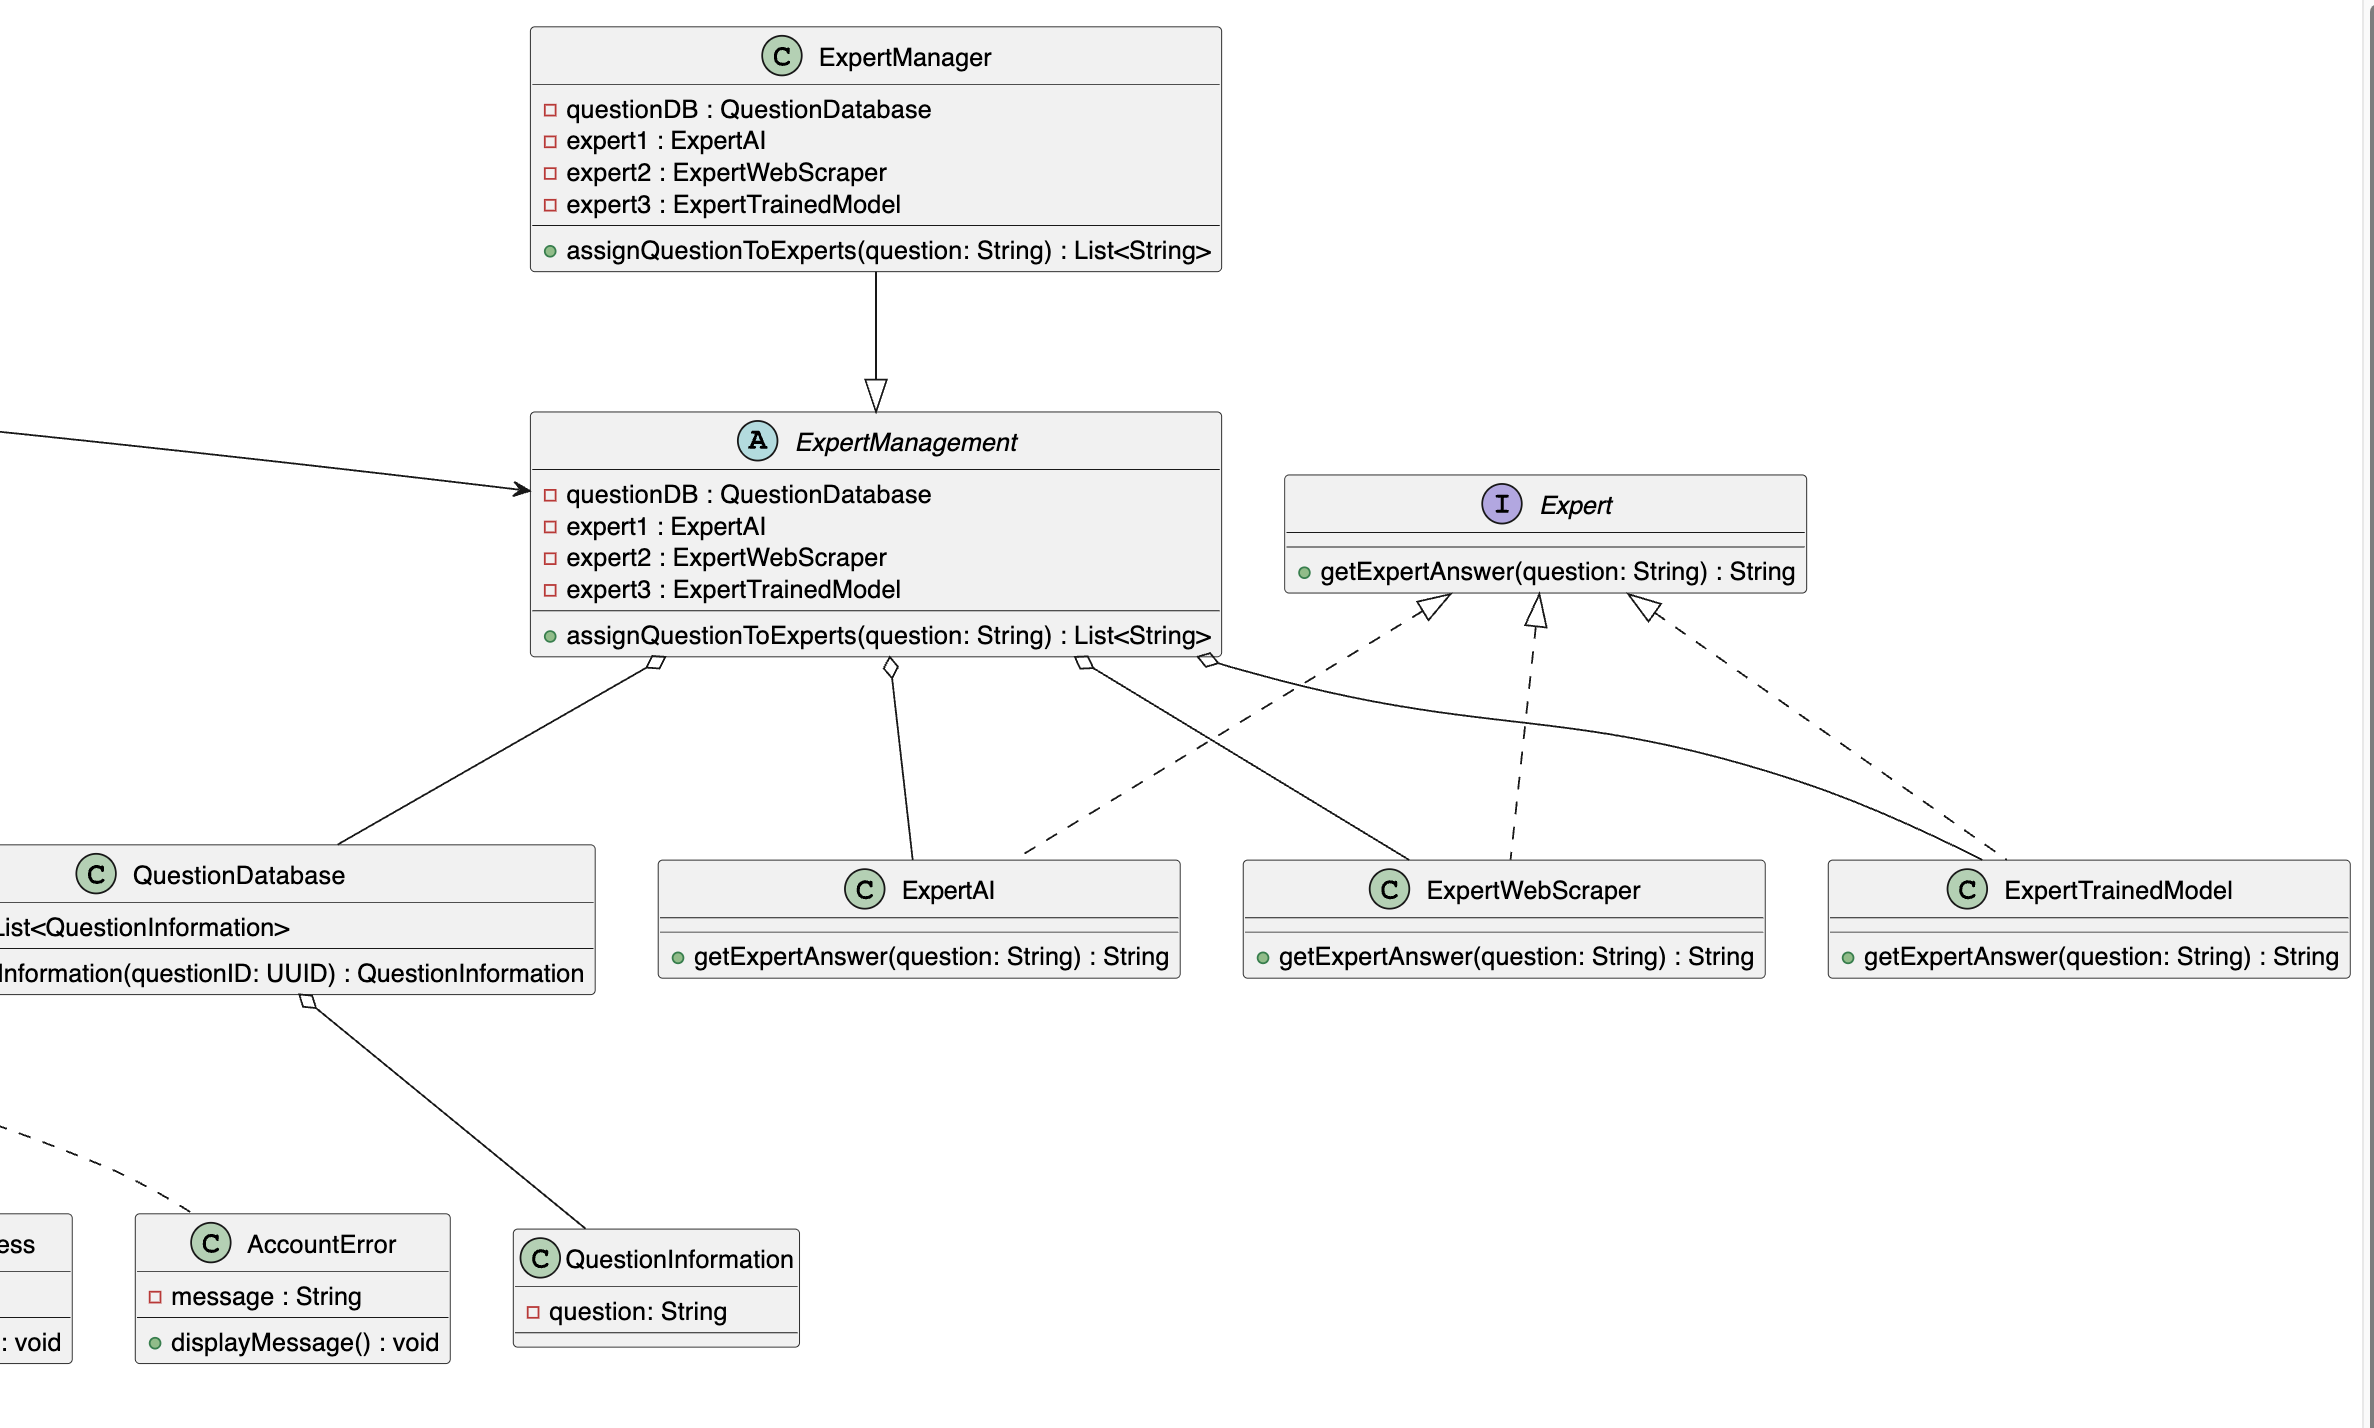
\includegraphics[width=1\textwidth]{diagrams/right.png} % Adjust width as needed
    \caption{Detailed Class Diagram 3 (Right)\\}
\end{figure}
% End Section

\clearpage
\appendix
\section{Division of Labour}
\label{sec:division_of_labour}
% Begin Section
Include a Division of Labour sheet which indicates the contributions of each team member. This sheet must be signed by all team members.\\

\noindent
\textbf{Patolia, Yash}
\begin{itemize}
	\item Section 1.2
	\item Section 1.3
	\item Sequence Diagrams: Login, Rating Sequence
	\item Compiled the entire document in LaTeX
\end{itemize}


\includegraphics[width=0.2\textwidth]{signatures/yash.png} % Adjust width as needed

\noindent
\textbf{Wang, Jasmine}
\begin{itemize}
	\item State Charts: Question Management, Expert Management
\end{itemize}


\includegraphics[width=0.2\textwidth]{signatures/Jasmine_signature.jpg} % Adjust width as needed

\noindent
\textbf{Kwinecki, Justin Joseph}
\begin{itemize}
	\item Section 1.1
	\item Sequence Diagrams: Edit Account, Create Account
\end{itemize}


\includegraphics[width=0.3\textwidth]{signatures/Justin.png} % Adjust width as needed

\noindent
\textbf{Zhang, Christina}
\begin{itemize}
	\item State Charts: Account Management
	\item Sequence Diagrams: Delete Question 
\end{itemize}


\includegraphics[width=0.2\textwidth]{signatures/ChristinaSignature.png} % Adjust width as needed

\newpage
\noindent
\textbf{Huzaifah, Muhammad}
\begin{itemize}
	\item State Charts: User Success Management
	\item Sequence Diagrams: Ask a Question
\end{itemize}


\includegraphics[width=0.2\textwidth]{signatures/Muhammad_Signature.png} % Adjust width as needed

\noindent
\textbf{Hum, Nathan Joshua}
\begin{itemize}
	\item Detailed Class Diragram
\end{itemize}


\includegraphics[width=0.2\textwidth]{signatures/NathanHumSignature.png} % Adjust width as needed
% End Section

\clearpage
\section*{IMPORTANT NOTES}
\begin{itemize}
	\item You do \underline{NOT} need to provide a text explanation of each diagram; the diagram should speak for itself
	\item Please document any non-standard notations that you may have used
	\begin{itemize}
		\item \emph{Rule of Thumb}: if you feel there is any doubt surrounding the meaning of your notations, document them
	\end{itemize}
	\item Some diagrams may be difficult to fit into one page
	\begin{itemize}
		\item It is OK if the text is small but please ensure that it is readable when printed
		\item If you need to break a diagram onto multiple pages, please adopt a system of doing so and throughly explain how it can be reconnected from one page to the next; if you are unsure about this, please ask me
	\end{itemize}
	\item Please submit the latest version of Deliverable 1 and Deliverable 2 with Deliverable 3
	\begin{itemize}
		\item They do not have to be a freshly printed versions; the latest marked versions are OK
	\end{itemize}
	\item If you do \underline{NOT} have a Division of Labour sheet, your deliverable will \underline{NOT} be marked
\end{itemize}


\end{document}
%------------------------------------------------------------------------------